\section{Anisotropías}

\subsubsection{Características del conjunto de datos del reporte}

\begin{itemize}
	\item Energía entre  [1 EeV , 2 EeV)
	\item Rango de tiempo:
	\begin{itemize}
		\item[-] Inicial:1388577600 (Thursday, 1 January 2014 12:00:00 GMT)
		\item[-] Final: 1577880000  (Thursday, 1 January 2020 12:00:00 GMT)
	\end{itemize}
	\item Sectancia:  $\theta < 60^o$
	\item 6T5
	\item $ib=1$ Bad period flag. Un valor de 1 indica un buen periodo
	\item Número de eventos: $1\,081\,844$
\end{itemize}


\begin{figure}[H]
	\centering
	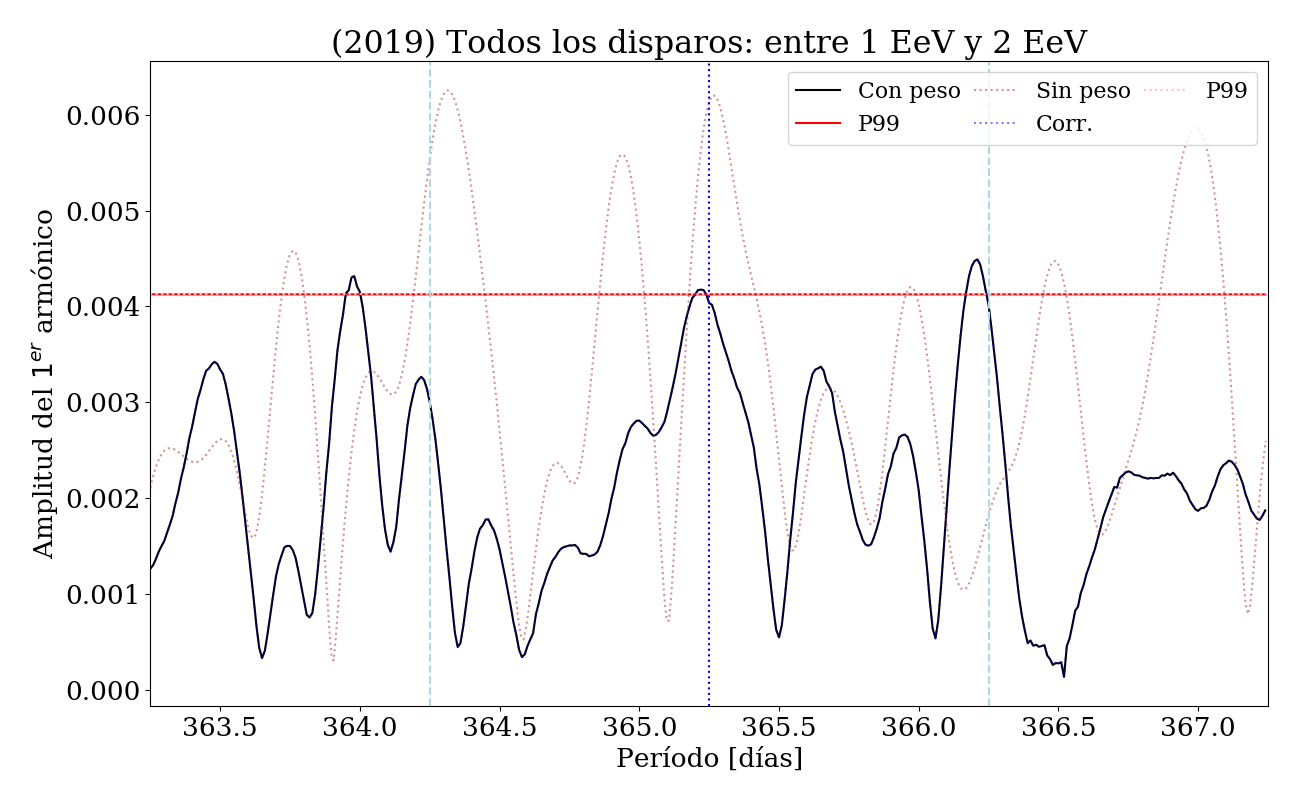
\includegraphics[width=0.8\linewidth]{../report_4_12_05_2020/2019_AllTriggers_1_2_EeV_con_vs_sin_peso.png}
	\caption{Anisotropía para el intervalo 2014-2020}
	\label{fig:anis}
\end{figure}

\begin{table}[H]
\centering
\begin{tabular}{l|c|c}
				& Con Peso 	& Sin peso 		\\ \hline
Frecuencia:		& 366.25 	& 366.25 		\\
Fase:			& 329.865 	& 292.312		\\
$P(r)$:			& 0.76398\%	& 26.6838 \% 	\\
Amplitud:		& 0.004676 	& 0.00243515	\\
\end{tabular}
\caption{Fase, $r_{99}$ y $P_{99}$ del análisis de anisotropía entre en 1 de Enero del 2014 y el 1 de Enero del 2020}
\end{table}



En la Fig.\ref{fig:zoom} se muestra el pico que se presenta en  el intervalo de energía entre 1 EeV - 2 EeV, cercano a la frecuencia sidérea. El pico tiene un máximo para un período de $366.21$. En la Tabla.\,\ref{tabla:pico} se muestran los valores de la fase, $r_{99}$ y $P_{99}$ para el periodo anterior.

\begin{figure}[H]
	\centering
	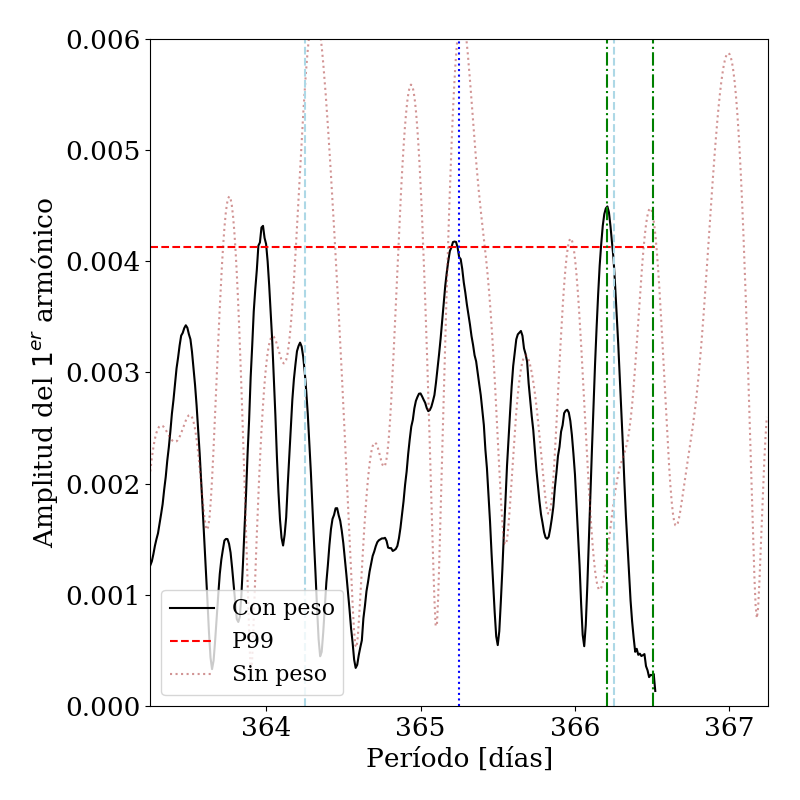
\includegraphics[width=0.5\linewidth]{zoom_anis.png}
	\caption{Zoom en el pico de anisotropía cercana para la frecuencia sidérea para el intervalo 2014-2020}
	\label{fig:zoom}
\end{figure}



\begin{table}[H]
\centering
\begin{tabular}{l|c|c|c|c}
				& Con Peso 		& Sin peso 		& Con Peso 		& Sin peso 		\\ \hline
Frecuencia:		& 366.21 		& 366.21 		& $\sim$366.505 & 366.506 		\\
Fase:			& 151.032 		& 121.695		& $\sim$190 	& 73.8188		\\
$P(r)$:		& 0.289882\%	& 46.9691 \% 	& $\sim$96\%	& 0.24013 \% 	\\
Amplitud:		& 0.00512146	& 0.0018417		& $\sim$0.0006	& 0.00520328	\\
\end{tabular}
\caption{Fase, $r_{99}$ y $P_{99}$ del análisis de anisotropía entre en 1 de Enero del 2014 y el 1 de Enero del 2020}
\label{tabla:pico}
\end{table}


\section{Ajuste del primer armónico de la variación de hexágonos y pesos}

Para verificar los valores de amplitud y fase en la frecuencia sidérea, se ajusta una función del tipo 
\begin{equation}
	f(RA) = a\cos{(2\pi(\omega RA + \phi))} +c
\end{equation}

a la variación de los hexágonos por ángulos de ascensión recta $RA$, así como también a la variación de los pesos de los eventos en ascensión recta \footnote{El peso de los eventos es la inversa del peso de los hexágonos}. En el ajuste, se dejan libres los parámetros de la amplitud $a$, desfase $\phi$ y offset $c$, en cambio la frecuencia $\omega=1$, ya que los valores de ascensión recta $0^o$ y $360^o$ son equivalentes y estamos trabajando con el primer armónico. La variación y el ajuste puede verse en las Figs.\ref{fig:pesos_ajuste} y \ref{fig:pesos_hexagonos}.

\begin{figure}[H]
	\centering
	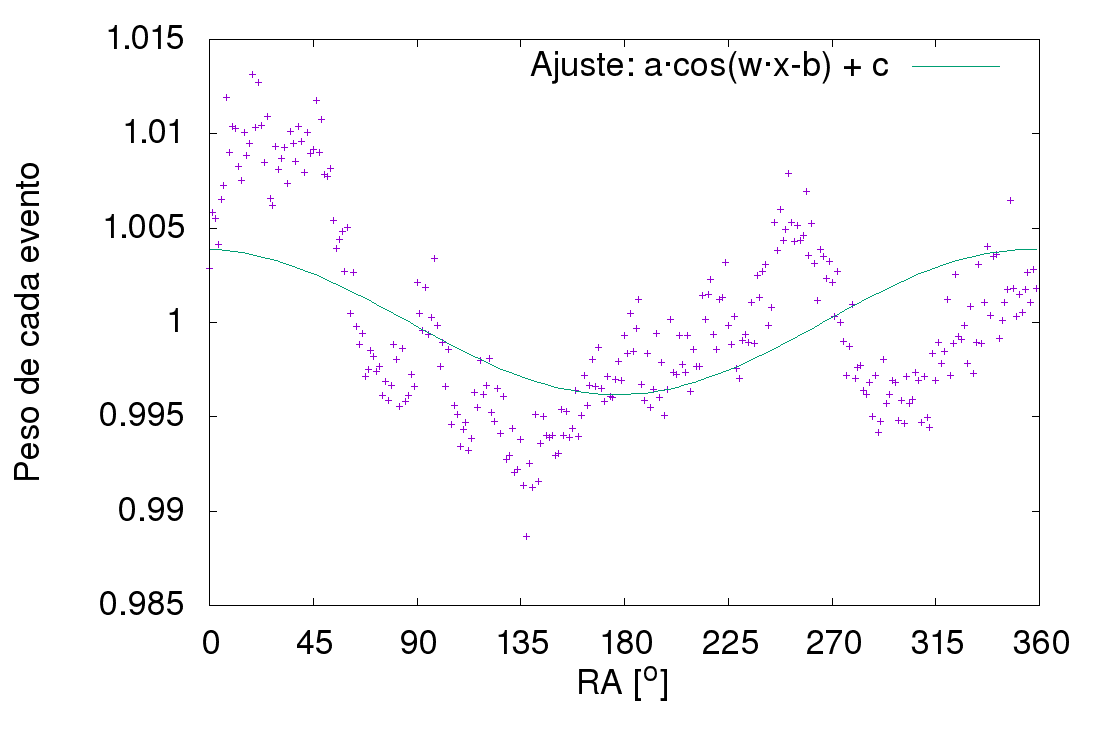
\includegraphics[width=0.5\linewidth]{ajuste_pesos.png}
	\caption{Pesos de los eventos en función de la ascensión recta para la frecuencia sidérea en el periodo 2014-2020}
	\label{fig:pesos_ajuste}
\end{figure}


\begin{figure}[H]
	\centering
	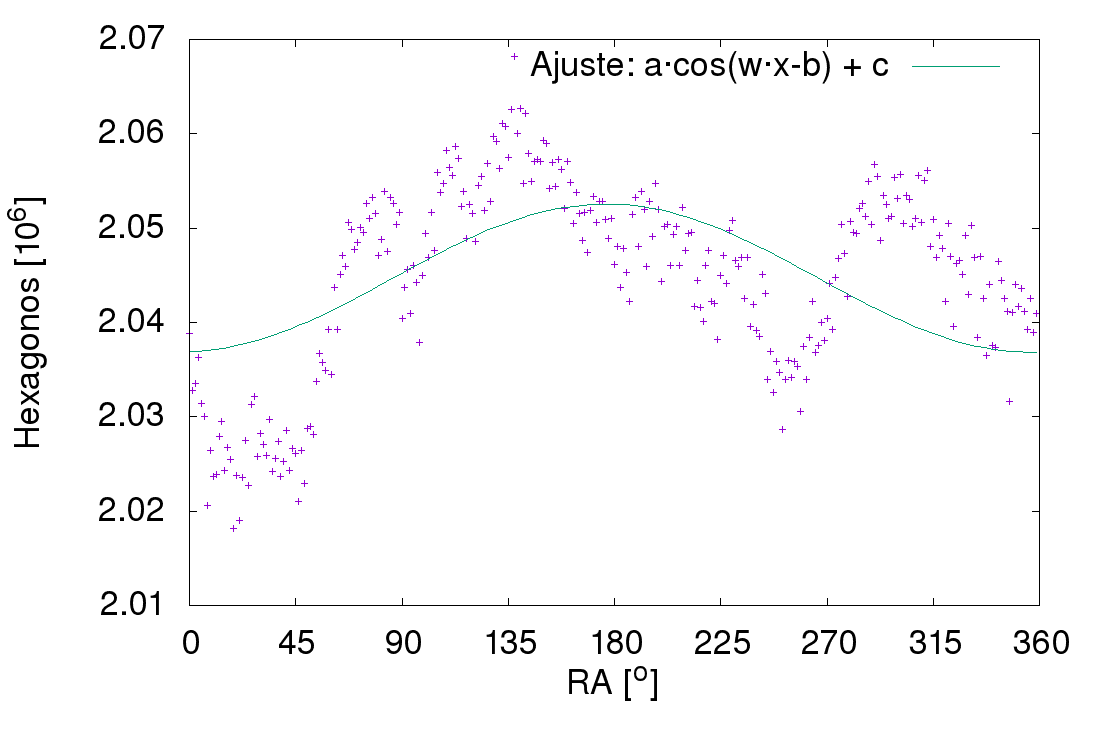
\includegraphics[width=0.5\linewidth]{ajuste_hexagonos.png}
	\caption{Hexágonos para la frecuencia sidérea en el periodo 2014-2020}
	\label{fig:pesos_hexagonos}
\end{figure}


Los valores de los ajustes, comparados con el análisis de Rayleigh se muestran en la Tabla\,\ref{tabla:ajuste_primer_armonico}. SE observa que el valor de la amplitud para el caso de la variación de los pesos es más cercana al que se obtuvo en el análisis de Rayleigh. Esto puede deberse que los pesos están normalizados por la integral de todos los hexágonos dada un frecuencia, por lo que si existe alguna constante multiplicativa en la cantidad de hexágonos, la amplitud la tabla para la primera columna puede no ser igual a la segunda columna.

\begin{table}[H]
\centering
\begin{tabular}{l|c|c|||c}
				& Hexágonos 				& Pesos	de los eventos		& Rayleigh con peso \\ \hline
Figura:			& \ref{fig:pesos_hexagonos} &\ref{fig:pesos_ajuste}		&\ref{fig:zoom} \\
Fase $\phi$:	& 284.874 	 				& 285.099					&329.865	\\
Amplitud $a$:	& 0.00784107 				&  0.00384774 				&0.004676\\
\end{tabular}
\caption{Fase y amplitud del ajuste del primer armónico en ascensión recta en los hexágonos y  pesos  de los eventos para la frecuencia sidérea}
\label{tabla:ajuste_primer_armonico}
\end{table}
